\chapter{Data Structures}

What exactly are data structures? Why would you use them? As the name implies, data structures are ways of handling information and values in an efficient manner in order to improve computational speed. Typically, they are used to store lots of values that are somehow related instead of having to create a normal variable for each one. Good knowledge of data structures is essential to being able to solve a problem in the fastest amount of time possible.

In most cases, you won’t ever have to write a data structure from scratch unless you are building a custom one tailored to fit a problem or are doing it to better learn the theory. Almost all languages will have have very efficiently written implementations in their libraries and all you have to do is to know which one works the best for your situation.

\section{Arrays}

Arrays are the simplest of data structures. They are a bunch of objects put in some order and stored in the memory. This is a big advantage over normal variables because if you wanted to store something such as the alphabet, one array could contain all of this information efficiently instead versus 26 different variables. Arrays are best for querying information. For example, if I wanted to know what the 14th letter was, I can do this in $O(1)$ time. However, if I want to add or remove something, arrays become very cumbersome as they have a fixed length. This means I have to create a second array and copy all of the information into this second one, adding or deleting any information I would like to change.

\section{ArrayList or Dynamic Array}

As mentioned above, arrays arrive at problems when information wants to be added or removed in an efficient manner. ArrayLists, otherwise known as Dynamic Arrays, attempt to solve this by sacrificing memory for computational speed. When an ArrayList is created, it will store more space than is needed. So for example if I wanted to store the names of all of my friends and had 13 of them, when I create an ArrayList while it will appear to me as if there are only 13 slots, the library running in the backend will actually create 16 slots and leave the extra ones as null (the smallest power of 2 greater than the length I ask for). Now, when I want to add a new friend I have made, the ArrayList will increment its displayed size and turn one of the next null slots into a person. It can conversely do the opposite for removing a friend. In this way, ArrayLists allow for $O(1)$ addition and subtraction for most cases, only occasionally being $O(n)$ when the length has to be expanded. This would happen if I were to go beyond 16 friends in the previous example, in which case a new array of length 32 would be created. This is limited however to adding or removing from the end, as otherwise all the elements have to shifted to fill gaps, therefore being $O(n)$.

\section{Linked Lists}

A list is a set of items that have some way of sorting themselves linearly. For example, if I was creating a list of numbers, they would be sorted by size yielding something such as 0, 1, 2, etc. In computer science, each item in a list is called a node. Each node has its value and a pointer, which references its neighbors. A good way to visualize this is a bunch of people in a line. Each person in the line knows what their name is and can also ask either of their neighbors for their name, but cannot directly ask anyone else.

So why do people use linked lists? Well ArrayLists are very effective in removing things from the end, but if items start being removed from the beginning then the data structure quickly becomes very messy. In addition, removing from the middle requires a lot of shifting as mentioned above. However, linked lists can add and remove in $O(1)$ time as a node simply has to change its pointer. For example, in the case of the line of people where person A is in front of B who is in front of C, if person B was to leave, then person C would simply treat the person in person A as the person in front of them instead of person B. However, the drawbacks of linked lists are that they take $O(n)$ time in retrieving data as each node must be iterated through before the target can be found.

As a side note, there are actually two types of linked lists. The more common one is a doubly linked list where a node will point to what is in front of it and behind it. On rare occasions, a singly linked list will be used where a node only knows what is in front of it in order to save memory.

\section{Stacks}

Stacks are an alternative method to storing data such that insertion and deletion is $O(1)$ but access is $O(n)$. A stack utilizes LIFO (last in, first out). Basically, it can be treated as a stack of books. If I was to put book A down, and then book B down on top of it, and so on all the way up to book Z, I would have a stack of books. Now if I wanted to take off a book, I would first have to remove book Z to look at anything below it. In this way, it becomes very cumbersome to retrieve previous items. However, stacks can be very useful in cases of where you only want to look at the last location. One example of this is in card games such as Pokemon or Magic: The Gathering. In these games, the last card to be played comes into play first, so that cards can be played to block other things. In such a case, all the cards are added to a stack time-sorted, and then resolved starting from the top of the stack. So if you were to play a card that said “You win the game!” and your opponent played a card that said “Ignore another card’s effect” in response to what you played, your opponent’s card would block your card and take effect first, preventing you from winning as the cards would be added to a stack.

\section{Queues}

A queue by contrast employs FIFO (first in, first out). This is similar to a line at a store, where the first person to begin waiting is the first person to be served by the counter. It also has $O(1)$ insertion and deletion and $O(n)$ querying like a stack, but is built to address different problems.

\section{Deque}

A deque, pronounced as deck, is a combination of a queue and a stack. Essentially, things can be added onto the back but can be removed from either the front or the back, utilizing either queue or stack principles depending on the situation. This can be useful in emulating games in which the rules often change, and therefore require a flexible data structure.

\section{Trees}
A tree is a non-linear data structure. Data in a tree is stored in “nodes.” Each node in a tree can have multiple successors/children, and all nodes (except the root) have exactly one predecessor. A leaf node is a node with no children. When a tree is drawn, the root is placed at the top, with arrows pointing to its child nodes. Here is an example tree: 

\begin{center}
\begin{tikzpicture}[very thick,level/.style={sibling distance=70mm/#1}]
\node [vertex] (r){\texttt{"a"}}
  child {
    node [vertex] {\texttt{"b"}}
    child {
      node [vertex] {\texttt{"d"}}
    }
  }
  child {
    node [vertex] {\texttt{"c"}}
    child {
      node [vertex] {\texttt{"e"}}
      child {node [vertex] {\texttt{"h"}}}
    }
    child {
      node [vertex] {\texttt{"f"}}
      child {node [vertex] {\texttt{"i"}}}
      child {node [vertex] {\texttt{"j"}}}
    }
    child {
      node [vertex] {\texttt{"g"}}
    }
  };
\end{tikzpicture}
\end{center}

\subsection{Binary Trees}
Generally, in a tree each node can have any number of children, but a binary tree is a specific type of tree in which each node has at most 2 children. [Note that a binary tree is different from a binary search tree (which is explained later) because the binary tree is not organized based on the values of the nodes.] The following is an example of a binary tree: 

\begin{center}
\begin{tikzpicture}[very thick,level/.style={sibling distance=70mm/#1}]
\node [vertex] (r){\texttt{"a"}}
  child {
    node [vertex] {\texttt{"b"}}
    child {
      node [vertex] {\texttt{"e"}}
    }
  }
  child {
    node [vertex] {\texttt{"d"}}
    child {
      node [vertex] {\texttt{"f"}}
      child {node [vertex] {\texttt{"i"}}}
      child {node [vertex] {\texttt{"h"}}}
    }
    child {
      node [vertex] {\texttt{"g"}}      
    }
  };
\end{tikzpicture}
\end{center}

In the tree above, “a” is the root, and “e”, “g”, “h”, and “i” are leaf nodes because they have no children. 

The tree has various properties. The height of a tree (also called depth) is the number of links needed to get from the root to the node furthest away from the root. For example, in the example tree, “h” (or “i”) is furthest away from the root. If we trace the path between the root and “h”, [trace: a to d, d to f, f to h], 3 links are made so the height is 3. The width of the tree is the longest path from one leaf to another (without crossing a path more than once). In this tree, the path is from "e" to "h" (or "i") and the width is 5. 

Another property is the internal path length. To calculate the internal path length, we add up the path lengths from the root to each node. For the example tree, the path from the root to itself is 0. From the root to its immediate children is 1. If we do this for all the nodes and sum the paths, the internal path length is 14. 

Another property is the external path length. First of all, an external node is where a node does not exist but could be drawn. For example, a leaf node has 0 children, so there are 2 external nodes there. The external path length is the sum of the paths to each external node. The path to an external node that stems from “e” would have length 3. If we do that for all the external nodes and sum the lengths, the external path length is 22. 

\subsection{Binary Search Trees}
A binary search tree is a tree where every node is greater than every node in its left subtree and less than or equal to every node in its right subtree. To use a BST, we need to impose some kind of ordering on the elements stored. Typically with characters and strings, a lexicographic comparison is made. Because there is no definite bound on the number of elements of the tree, we typically create our own object or structure to represent the tree with left and right pointers. When searching for an element in the tree, we employ a binary search and find the element we desire in $O(log(N))$ time. Note that this time complexity is only for a well balanced tree. For example, if the tree's elements are strictly increasing, then the tree becomes more like a LinkedList structure (therefore $O(N)$ in the worst case). Below is an example of a Binary Search Tree:
\begin{center}
\begin{tikzpicture}[very thick,level/.style={sibling distance=70mm/#1}]
\node [vertex] (r){\texttt{"m"}}
  child {
    node [vertex] {\texttt{"g"}}
    child {
      node [vertex] {\texttt{"c"}}
      child {
        node [vertex] {\texttt{"b"}}
        child {node [vertex] {\texttt{"a"}}}
        child[missing]
      } 
      child {
        node [vertex] {\texttt{"e"}}
      }
    }
    child {
      node [vertex] {\texttt{"j"}}
      child {node [vertex] {\texttt{"h"}}}
      child {node [vertex] {\texttt{"k"}}}
    }
  }
  child {
    node [vertex] {\texttt{"t"}}
    child {
      node [vertex] {\texttt{"r"}}
      child[missing]
      child {node [vertex] {\texttt{"s"}}}
    }
    child[missing]
  };
\end{tikzpicture}
\end{center}


\section{Sets}
\subsection{Ordered Sets}
A set is a data structure that can be thought of as a bundle of unique elements. There are two distinct types of sets: one that retains order and one that does not. If a set has order, it is typically ordered in the form of a tree. In Java this is referenced as an TreeSet and in C++ it is can be invoked by std::set. In an ordered set, look up is typically $O(log(N))$ where $N$ is the total number of elements in the set. The logarithm comes from the nature of the tree being used to keep track of the ordering of the set. Below you can see an example of an ordered set in Java being represented through a tree-based structure.
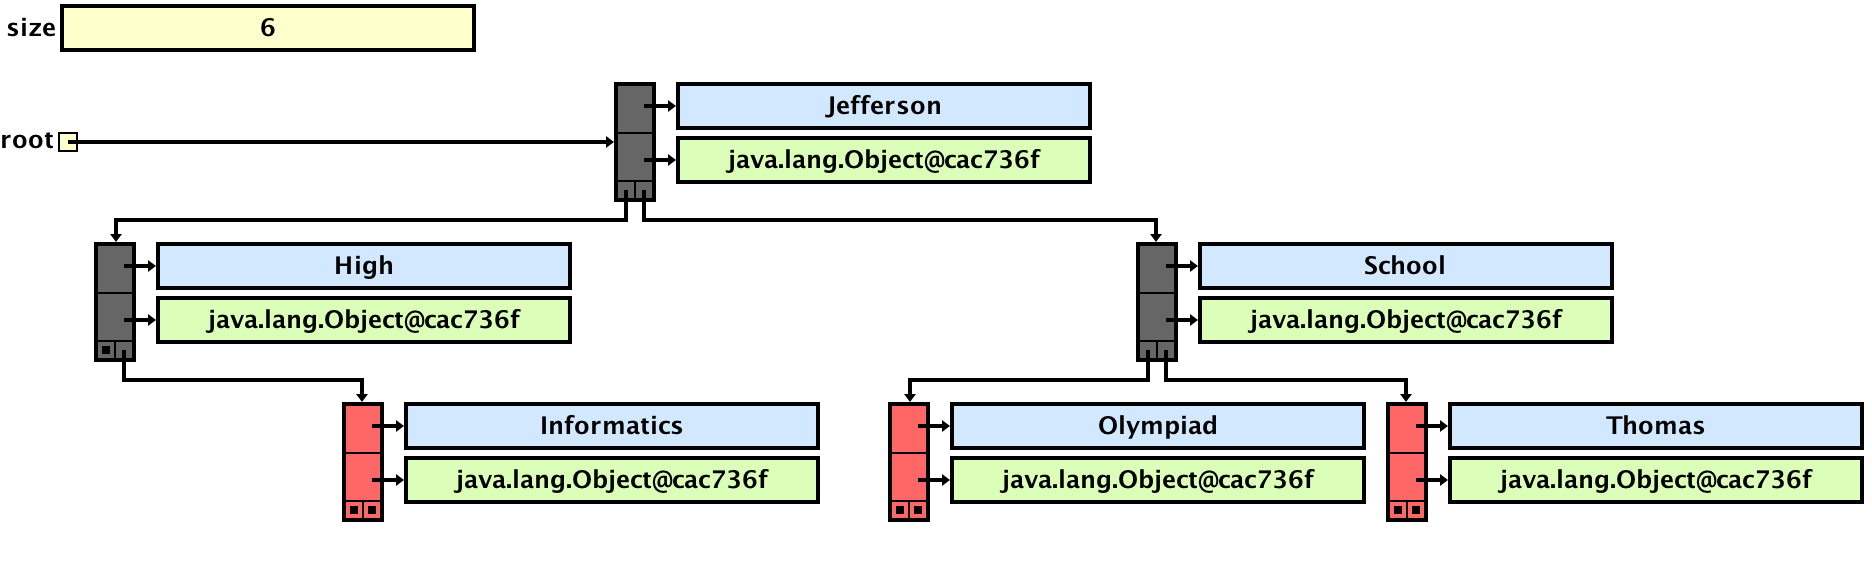
\includegraphics[scale=0.5]{treeset.png}
\subsection{Unordered Sets and Hashing}
A set without ordering is typically faster because of a wide-used trick known as Hashing. In brief, Hashing is a way of storing items so they can be found later on efficiently. The items are stored in a hash table at a position specified by a hash code. A hash code is an integer value calculated from any given data value or object, and is used to determine where a value should be stored in a hash table. This hash code value is generated by a hash function, a function that will always produce the same hash code given a specific data value or object. If two objects produce the same hash code, this is known as a collision. A collision is typically handled by creating buckets that contain LinkedLists. If there is a collision and there is intent to do a look up, the run time would increase as the program would still have to go through all of the elements in the bucket. Unordered Sets use this trick to attain their $O(1)$ look up. In Java unordered sets are referenced as HashSets and in C++ they can be invoked by std::unordered\_set. In the representation below, you can see the hash table for this particular unordered set (notice the collision at index 0).
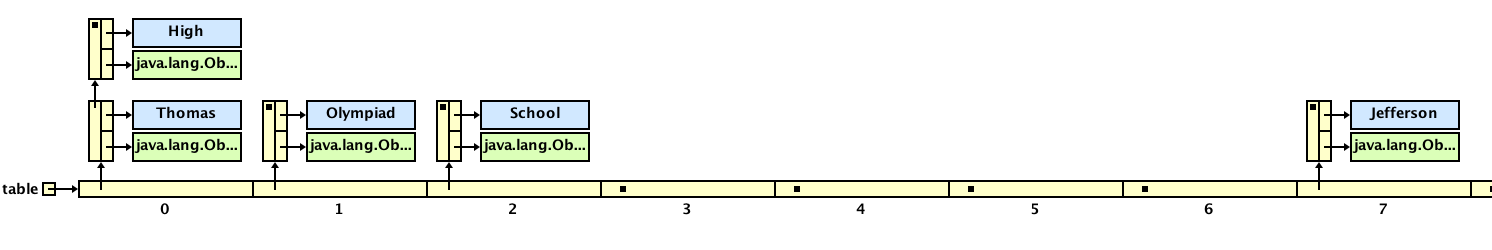
\includegraphics[scale=0.64]{hashset.png} 


